\documentclass{article}
%packages
\usepackage{graphicx}
\usepackage[utf8]{inputenc}
\usepackage[T1]{fontenc}
\usepackage[frenchb]{babel}
\usepackage[a4paper]{geometry}
\usepackage{minted}
\usepackage{hyperref}

\begin{document}
%title
\begin{titlepage}
	\vspace{-20px}
	\begin{tabular}{l}
		
\includegraphics[scale=0.1]{esir.png}\\
		\\
		\textsc{Blin} S\'ebastien\\
		ESIR 1 - Informatique\\
		2014-2015\\
		\\
		\textsc{Engel} Jean-Christophe\\
		Maître de conférences à l'ESIR
	\end{tabular}
	\hfill
	\begin{tabular}{l}
		
\includegraphics[scale=0.5]{telecom}\\
		Télécom Bretagne\\
		2 Rue de la Châtaigneraie,\\
		35510 Cesson-Sévigné\\
		+33 2 99 12 70 00\\
		\\
		\textsc{Toutain} Laurent\\
		Maître de conférences\\
		Département RSM
	\end{tabular}
	\vfill
	\begin{center}
		\vspace{0.5cm}\hrule\vspace{0.5cm}
		\LARGE{\textbf{Rapport de stage}}\\
		\Large{Télécom Bretagne - Projet LoRa FABian}
		\vspace{0.5cm}\hrule
	\end{center}
	\vfill
	\begin{flushleft}
		\Large{Année universitaire 2014-2015}
		\hspace{4cm}
		
\includegraphics[scale=0.6]{univ}
	\end{flushleft}
\end{titlepage}

\begin{titlepage}
\vspace{\fill}
\begin{flushright}
Remerciements~:
TODO
\end{flushright}
\vspace{\fill}
\end{titlepage}

\thispagestyle{empty}
\tableofcontents
\listoffigures
\newpage
\setcounter{page}{1}

\section{Introduction}
\subsection{Descriptif du stage}
Durant 3 mois, j'ai contribué au projet LoRa FABian. Il s'agit d'un projet visant à offrir des technologies libres et standardisées pour les besoins de communication des objets communicants (IoT,- Internet of Things). Le réseau est inspiré des réseaux multi-tiers 3G/4G. Il est constitué de quatres entités. Le noeud F(ar) est l'objet communicant. Il communique via ondes radios (norme 802.15.4) à un noeud R(adio). Les antennes sont ensuite reliées à un noeud G(ateway) qui communique en HTTPS à un noeud S(ervice).\\
L'objectif du stage était d'améliorer les implémentations des noeuds F, c'est-à-dire d'améliorer le shield de la société Wi6labs ainsi que la librairie Arduino dans le but d'offrir une implémentation ouverte, facile à prendre en main et documentée.
\subsection{Télécom Bretagne}
\subsection{Objectifs personnels}
Ce stage était pour moi une occasion de découvrir ce qu'était le travail sur un projet en tant qu'Ingénieur de Recherche dans un laboratoire. De plus j'ai pu découvrir quelques problématiques d'un projet d'entreprise open-source (notament la question de la licence de publication des morceaux de codes et les choix technologiques) et de découvrir le monde du travail dans le domaine de l'embarqué (hésitant actuellement entre une professionnalisation dans l'embarqué ou dans le Machine Learning en dernière année) (TODO plaquette ESIR)
\subsection{Plan}

\section{Bilan personnel}
\subsection{Découverte des outils}
Lors de ce stage, j'ai eu le besoin de prendre en main plusieurs outils.\\
Le shield de la société Wi6labs fonctionnent sur un environnement Contiki. Durant les 2 premières semaines et dans le but de découvrir l'environnement, j'ai aidé à la réalisation de deux différents TPs pour un cours d'été. Le premier TP consistait à contrôler des prises électriques fonctionnant sur Contiki via des requêtes COAP. J'ai eu besoin de flasher les cartes des prises électriques [Figure~: \ref{fig:progprise}] et du prendre en main la machine virtuelle Contiki (une machine virtuelle sous Ubuntu Linux avec des outils spécifiques à Contiki (Pour lister les devices, les flasher, etc.), ainsi que le dépot du projet contenant tous les fichiers sources).\\
La partie serveur pour envoyer les requêtes COAP via radio était une carte de type TMOTE-sky [Figure~: \ref{fig:tmotesky}]. Enfin l'application COPPER était installée sur les PC pour interargir avec les prises via le navigateur Mozilla Firefox.\\

\begin{figure}[h]
	\begin{center}
		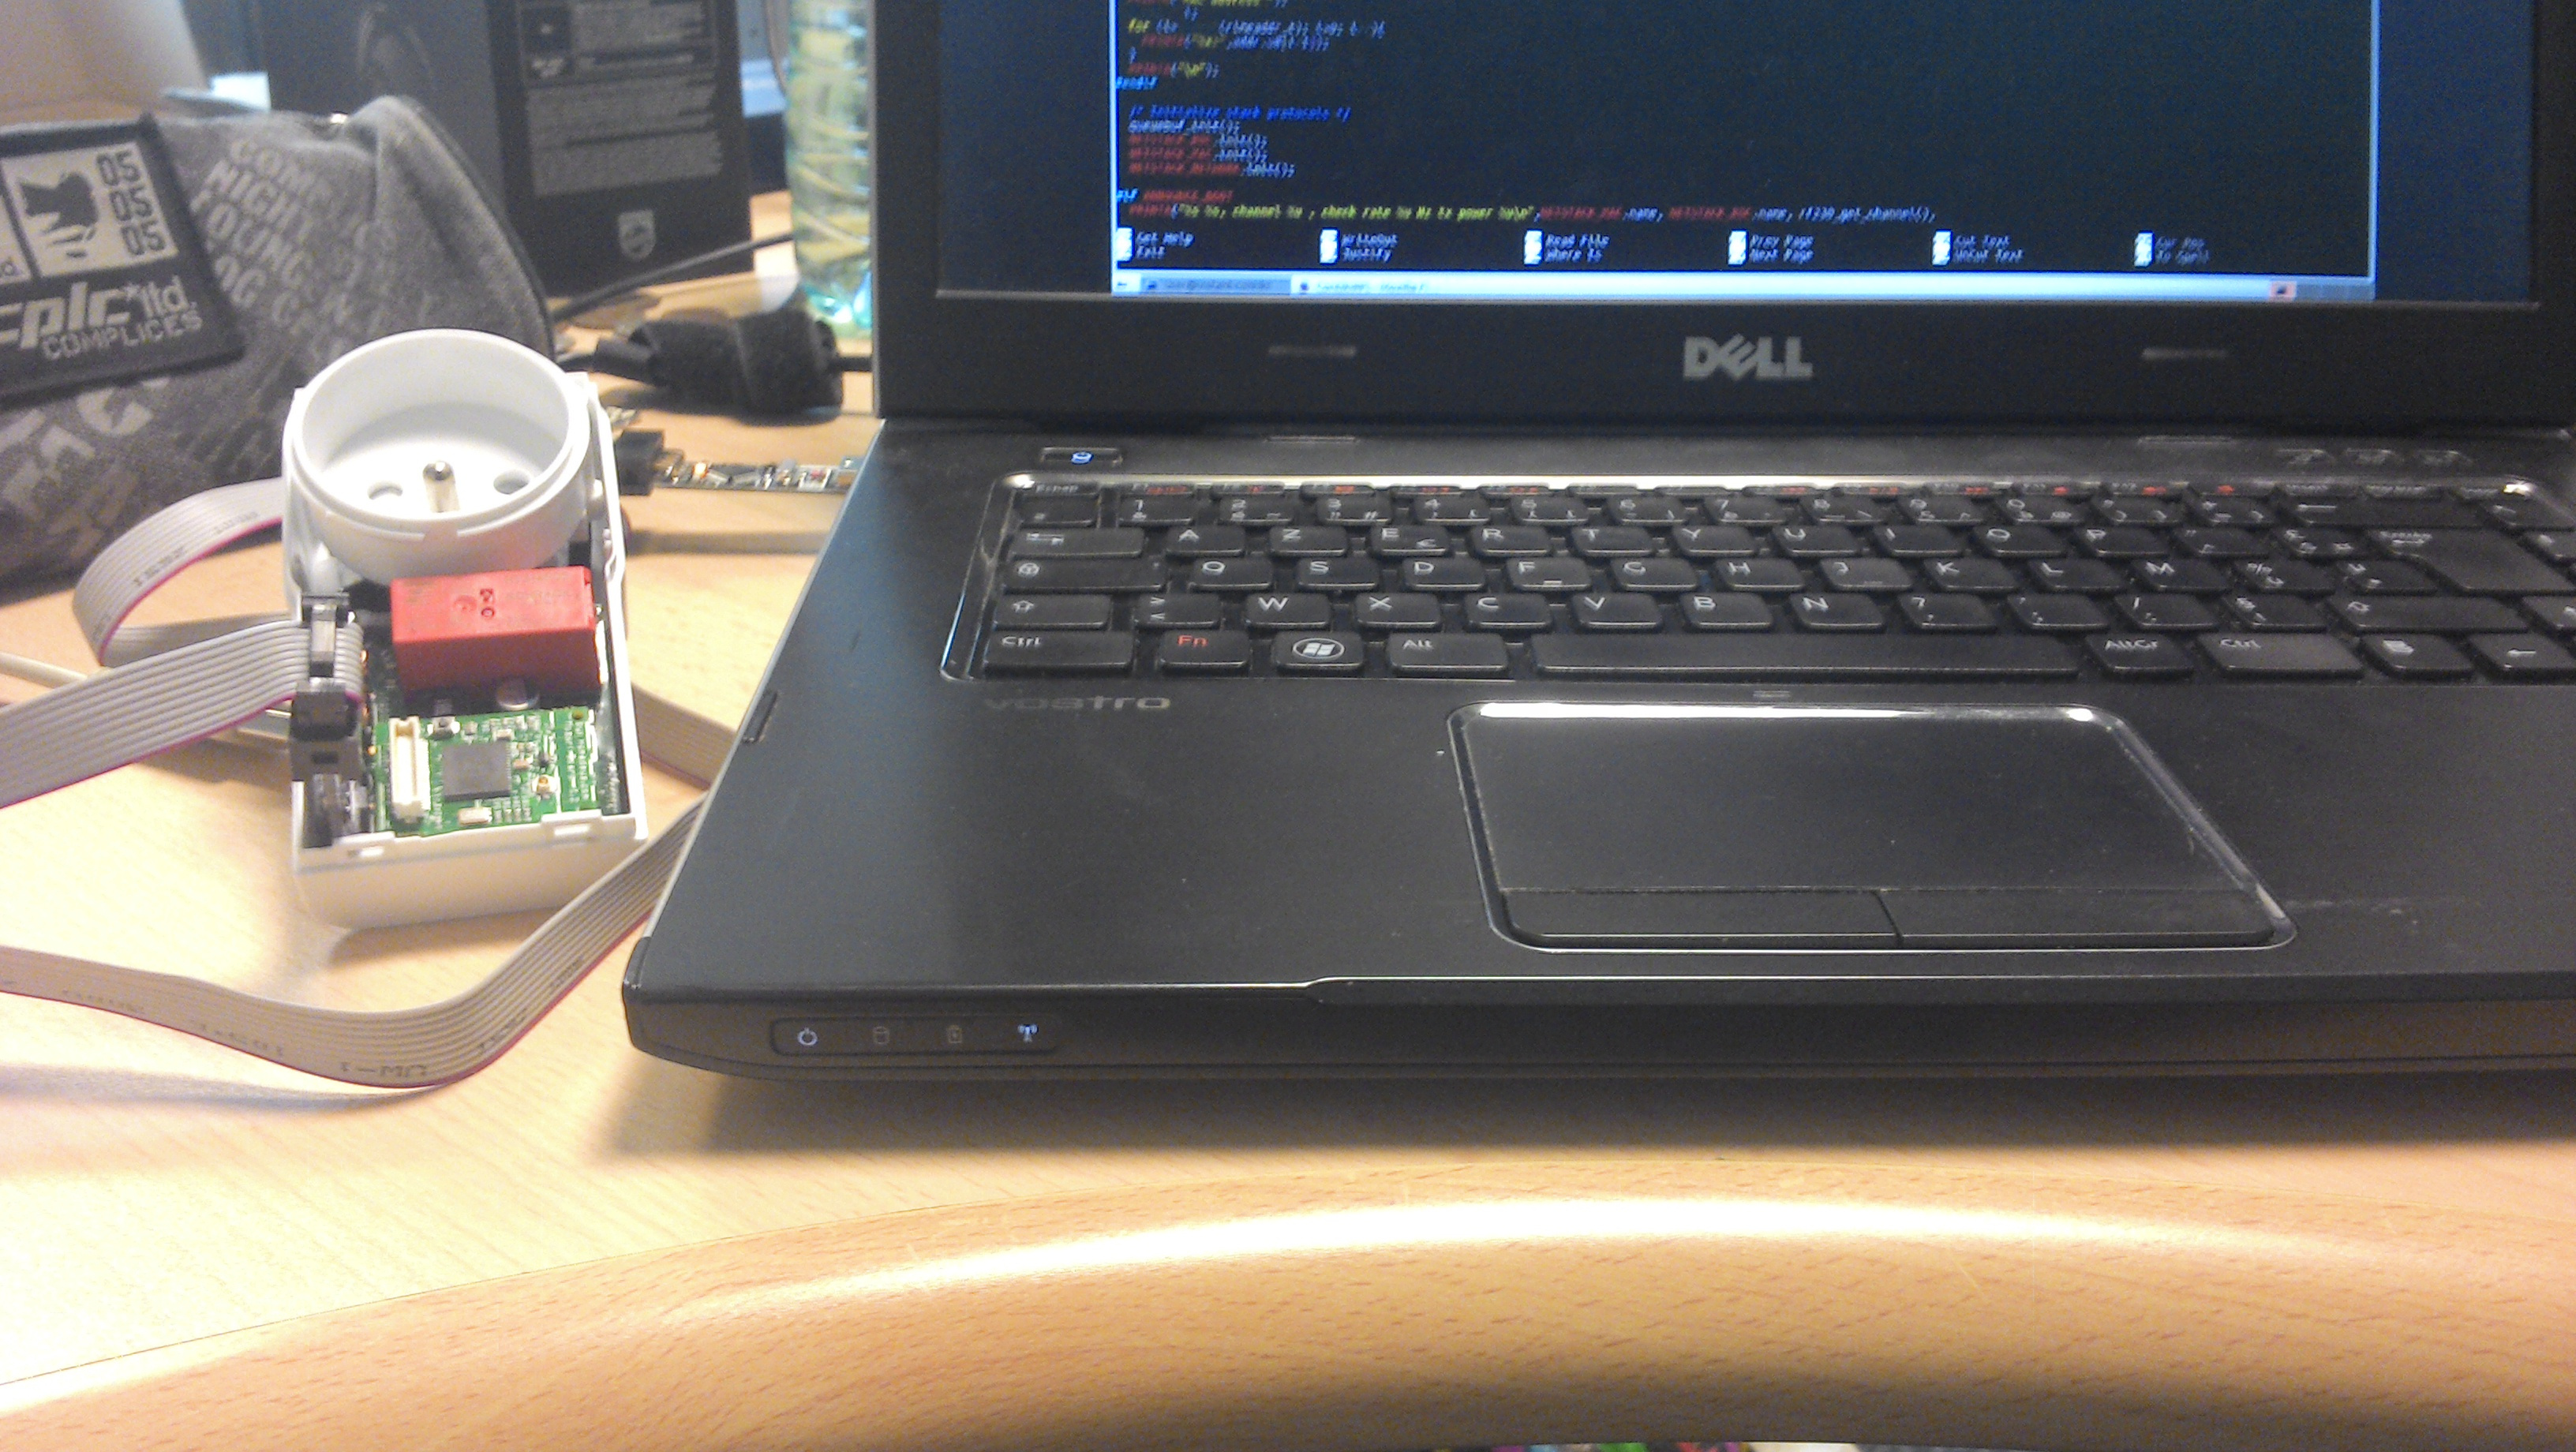
\includegraphics[scale=0.1]{../res/img/progprise.jpg}
		\caption{Programmation d'une prise sous Contiki OS}
		\label{fig:progprise}
	\end{center}
\end{figure}
\begin{figure}[h]
	\begin{center}
		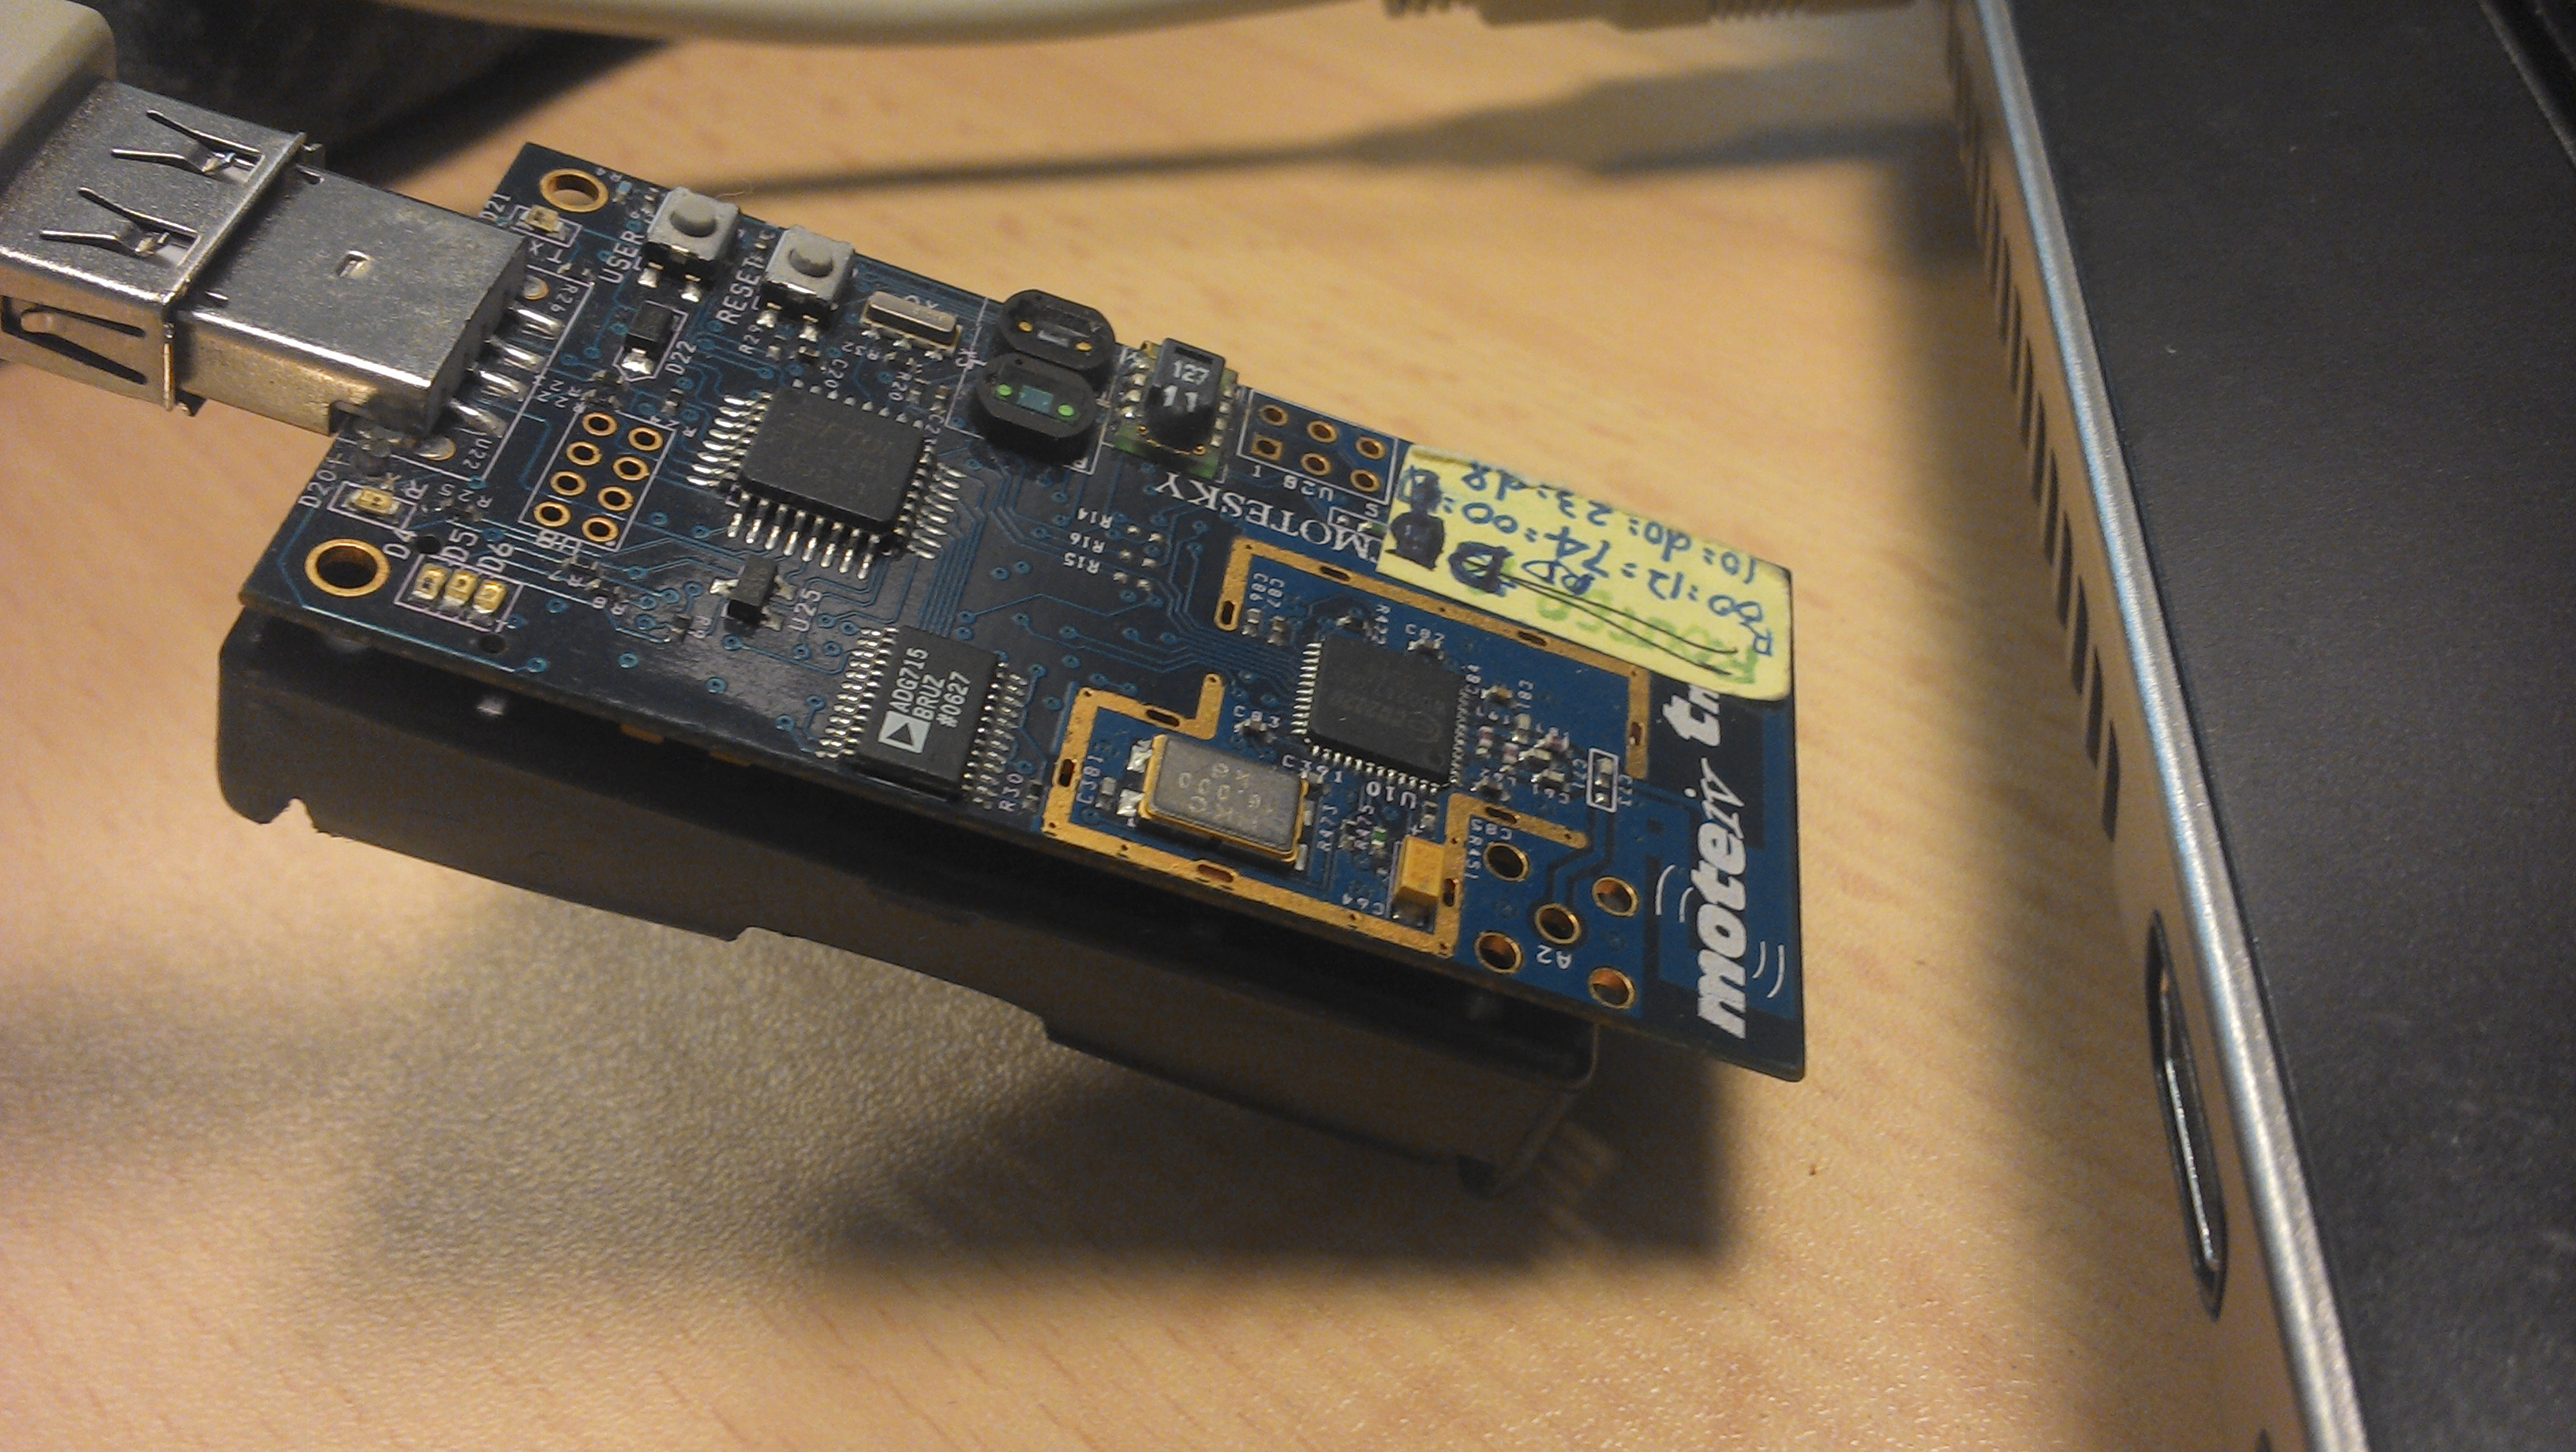
\includegraphics[scale=0.1]{../res/img/tmote.jpg}
		\caption{Carte TMote-sky}
		\label{fig:tmotesky}
	\end{center}
\end{figure}

Le second TP était la prise en main des shields LoRa pour Arduino. Le but étant de répondre à des requêtes COAP en renvoyant une page web avec un petit message, ou allumer une led, etc. Pour cette partie, j'ai donc du prendre en main le Shield ainsi que la carte TLink pour pouvoir flasher et debugguer le shield [Figure~: \ref{fig:shield}]. Pour la partie Arduino, j'ai du améliorer le code de la bibliothèque actuelle pour le rendre plus simple à comprendre et j'ai donc utilisé des cartes de type Arduino Uno.\\
Durant cette phase de découverte, la seule difficulté que j'ai rencontré était le manque ou l'inexactitude de la documentation sur des parties complètes du projet (le projet étant à la fois en développement et en phase de réflexion, la documentation n'est pas complète ou obsolète car la technologie a été modifiée).
\begin{figure}[h]
	\begin{center}
		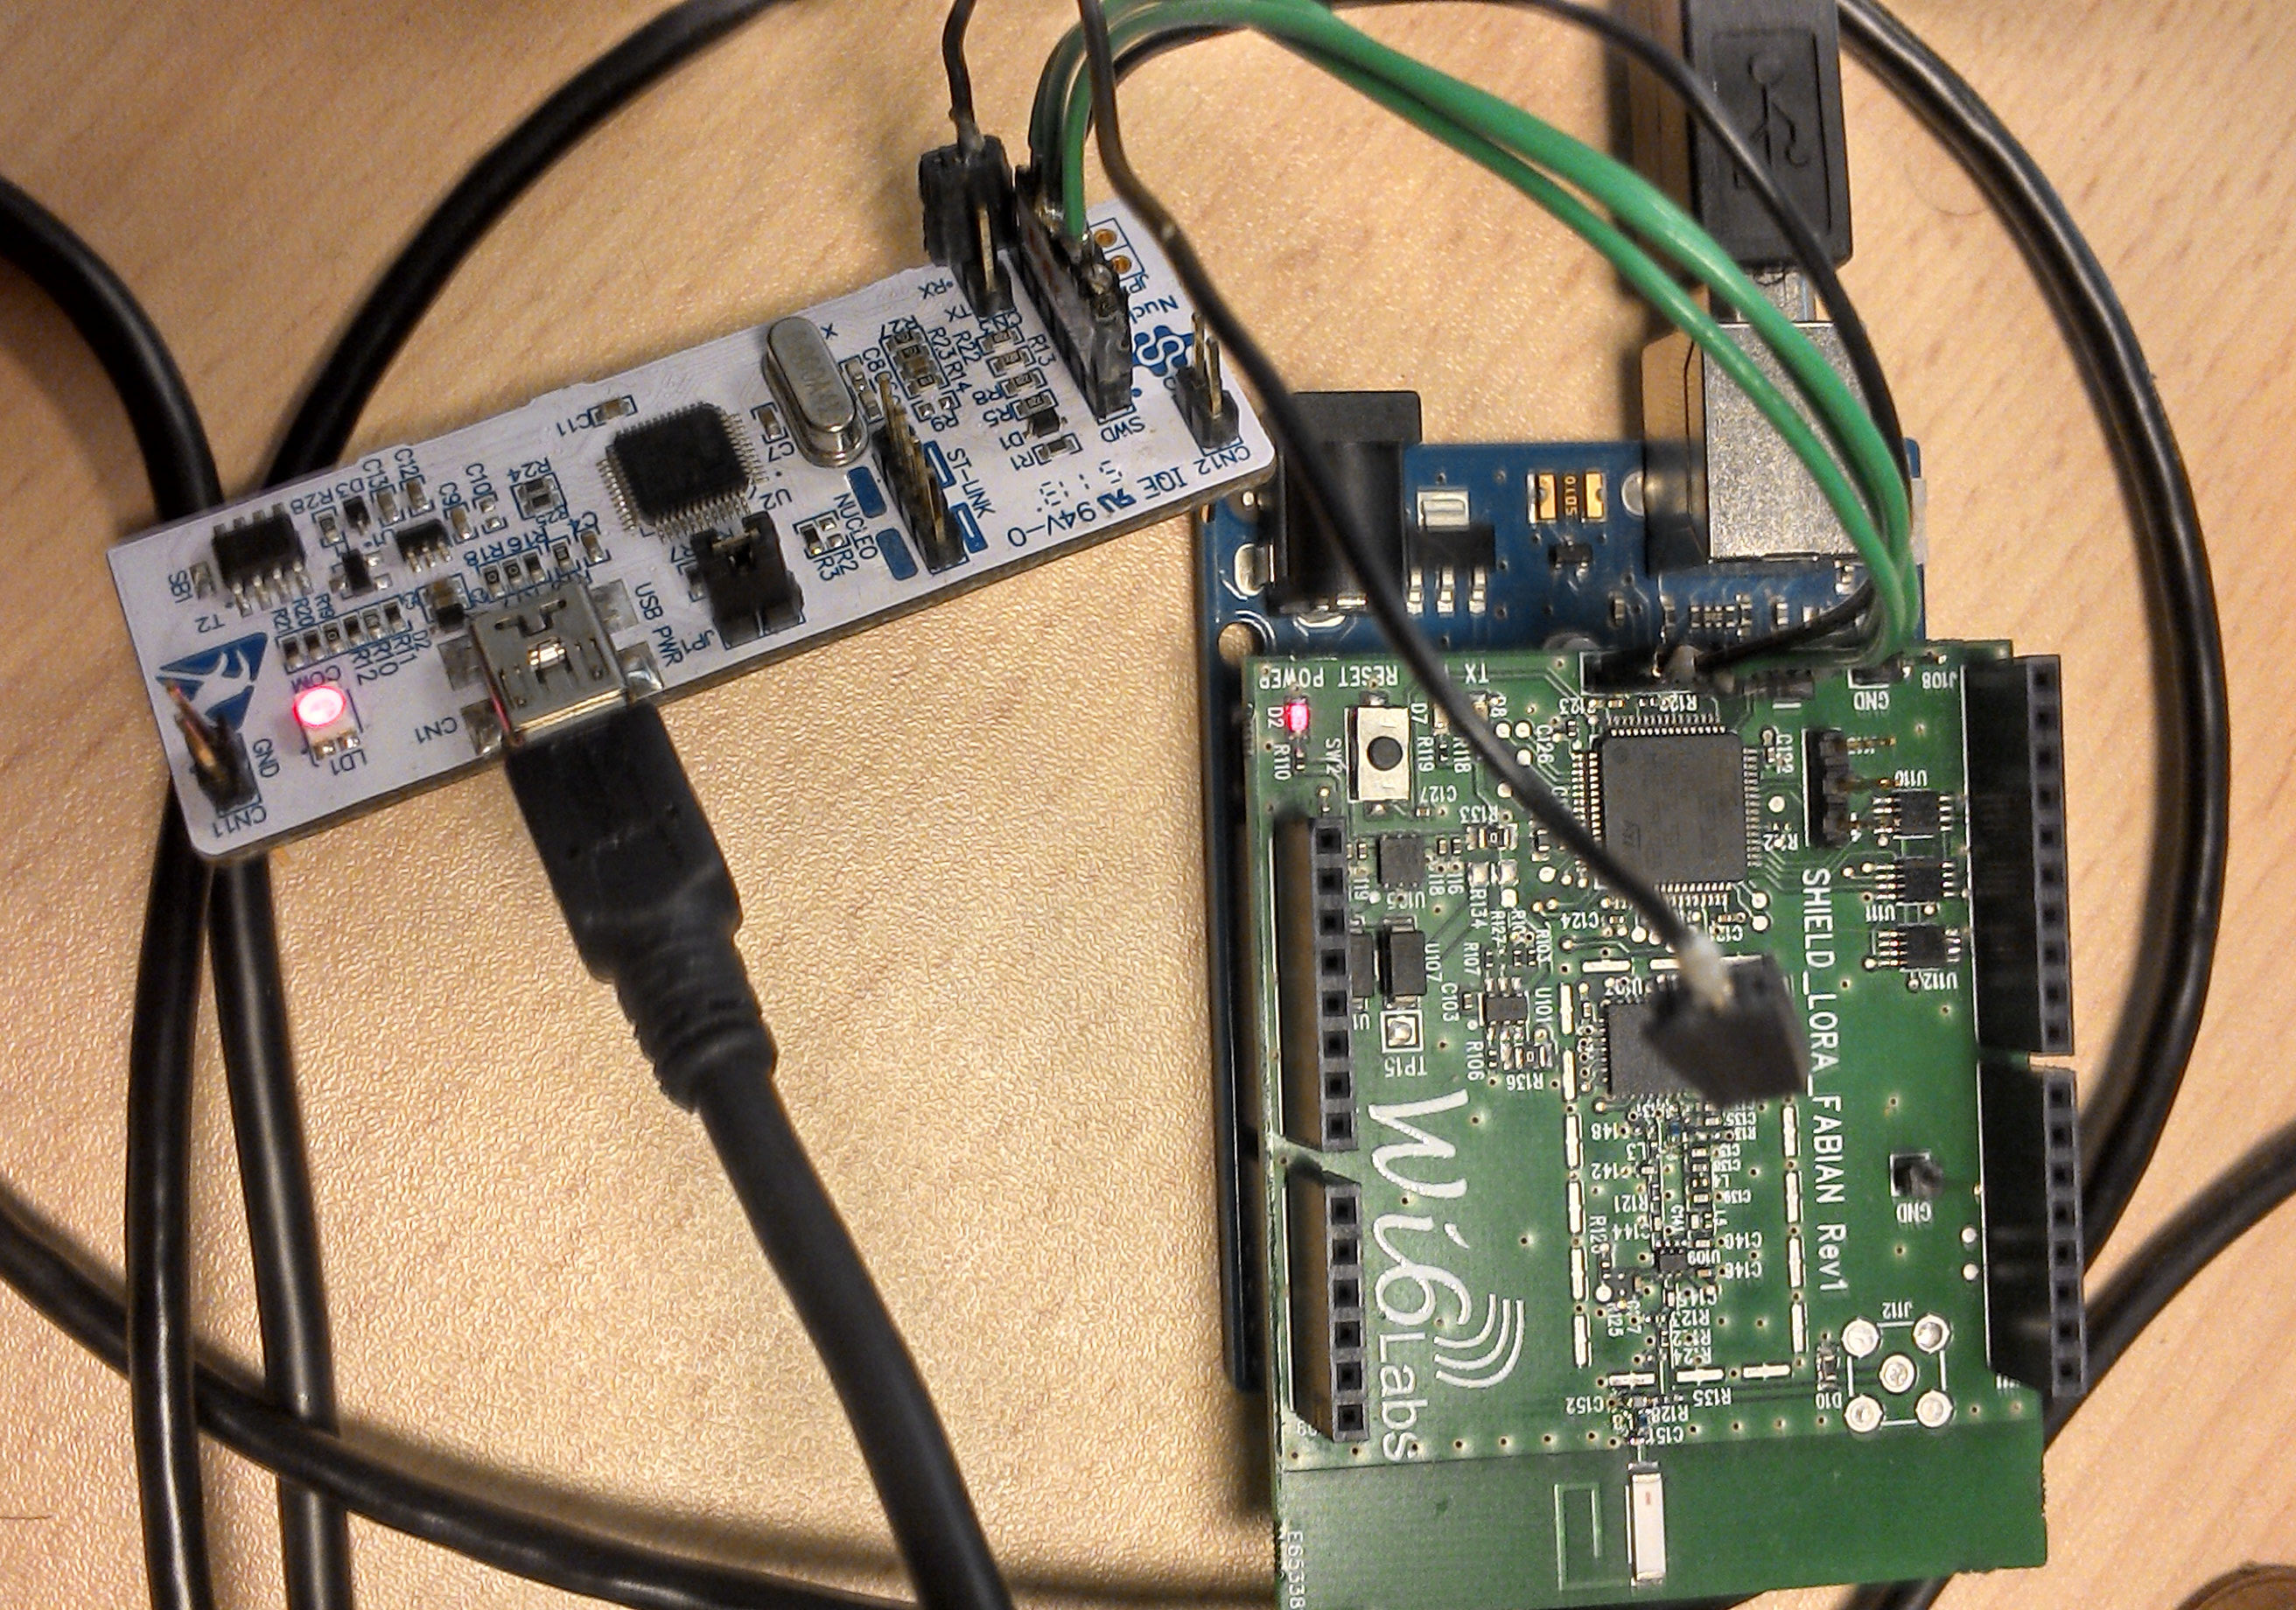
\includegraphics[scale=0.1]{../res/img/shield.jpg}
		\caption{Reprogrammation du shield de la société Wi6labs}
		\label{fig:shield}
	\end{center}
\end{figure}
\subsection{Mission principale}
TODO présenter architecture du projet
amélioration de la librairie arduino ~ du node F
bouger 802.15.4 sur la board contiki
beacon incremental backoff
refaire lib arduino
partie qui envoie à la carte.
difficultés : documentation incomplète (projet en développement), voir inexacte ou pas à jour car change très très vite.
\subsection{Méthodologie de travail}
Ce stage m'a permis de développer plusieurs compétences en rapport avec la méthodologie de travail.\\
En effet, j'ai du au fil des missions annexes et de la mission principale à la fois travailler en autonomie sur ma partie (modifier la librairie arduino, reprogrammer les cartes, enlever la stack 802.15.4 de la carte Arduino vers le shield Contiki) et travailler en équipe (ma partie étant utile à d'autres parties du projet, ou alors pour l'organisation des TPs).\\
Je me suis aussi trouvé en parfaite autonomie au niveau de mes horaires. En effet, aucun horaire n'était fixé. Lorsque je le pouvais, je commençais tôt le matin avec une veille informationnelle, puis je programmais ce dont j'avais besoin le matin. L'après midi étant souvent composée d'une phase de test + debug du code. Enfin je finissais ma journée par de la lecture de documentation et en préparant une TODO list pour les jours suivants.\\
Les missions annexes m'ont aussi permis de développer des compétences. En effet, j'ai pu contribuer à l'organisation de TPs pour des cours d'été (donc relecture du sujet, programmation des bibliothèques, préparation des cartes, tests en salle) ainsi qu'à la réalisation d'une conférence (modification du diaporama déjà existant, répartition du temps de parole, préparation du texte, présentation devant un public puis réponses à ses questions).
\subsection{Missions annexes}
Durant ce stage, j'ai aussi été amené à réaliser d'autres missions annexes. Par exemple, j'ai été co-intervenant à la conférence \emph{LoRa Fabian~:  projet visant à fournir des protocoles ouverts et standardisés pour les besoins de communication des objets communiquant (IoT)} avec Mathieu Goessens durant l'évènement \emph{Portes Ouvertes Ou Pas} à Paris. (Voir annexe A).

\section{Conclusion}
Tester une grande entreprise ?\\
Listing des compétences acquises\\
embarqué ou ML ?

\newpage
\appendix
	\section{Conférence~: Portes Ouvertes Ou Pas}
	L'évènement \emph{Portes Ouvertes Ou Pas} s'est déroulé à Paris (20 rue de Reuilly) le 13 \& 14 Juin 2015.
		TODO présentation de l'évènement + liens vers slides \& vidéo
\end{document}

